\documentclass[12pt,a4paper,titlepage,notitlepage]{article}
\usepackage[utf8]{inputenc}
\usepackage[T1]{fontenc}
\usepackage{amsmath}
\usepackage{amssymb}
\usepackage{makeidx}
\usepackage{graphicx}
\usepackage[width=0.00cm, height=0.00cm, left=3.00cm, right=3.00cm, top=3.00cm, bottom=3.00cm]{geometry}

\usepackage{tocbibind}
\usepackage{booktabs}
\usepackage{array}

\title{\textbf{Wireless Power Transfert} $\left( WPT\right)$. \vspace{5cm}}
\author{ \ \\Fait par: MATUMBA KANIKI Joed\\ \ \\ Directeur: Prof. Dr. Ir. Matthieu LIASSA NKOY LUTAKA-LUTAKA\\ \ \\ Co-Directeur: Ass. Ir. Elie BOTULI EBANZA\\ }

\date{\vfill \today }

\begin{document}
	\maketitle
	\newpage
	\tableofcontents
	
	\newpage
	\section*{Remerciements}
	\addcontentsline{toc}{section}{Rémerciements}
	\newpage
	
	\vspace{2cm}
	\section{Introduction}	
	\vspace{1cm}	
	Au cours des dernières décennies, la demande croissante pour des dispositifs électroniques portables et connectés a conduit à une évolution significative des technologies de transfert d'énergie. Le transfert d'énergie sans fil (WPT, pour \emph{Wireless Power Transfer}) s'est imposé comme une solution innovante et pratique, se débarrassant des contraintes physiques des câbles d'alimentation. Cette technologie, qui permet la transmission d'énergie électrique sans contact physique, trouve des applications variées allant de la recharge de dispositifs mobiles à l'alimentation de véhicules électriques, en passant par des applications biomédicales.\\
	
	L'un des principaux défis du WPT réside dans l'optimisation de l'efficacité de transfert d'énergie, surtout sur de longues distances. En effet, la distance entre l'émetteur et le récepteur, ainsi que l'alignement des bobines, influencent considérablement l'efficacité du transfert. Plusieurs méthodes, telles que la résonance magnétique et l'induction électromagnétique, ont été développées pour améliorer ce domaine. Grâce aux avancées en matière de matériaux et de systèmes de contrôle, le WPT a vu ses performances s'améliorer, répondant ainsi aux besoins d'une variété d'industries.\\
	
	
	Avec l'essor de l'Internet des Objets (IoT), où des millions d'appareils sont interconnectés via des réseaux sans fil, le WPT s'avère essentiel pour assurer l'autonomie énergétique de ces dispositifs. Grâce à des normes de sécurité et des technologies innovantes, le WPT est non seulement une solution pratique mais également une avancée vers une énergie plus durable et accessible.\\
	
	%% Les techniques de transfert d'énergie sans fil ont attiré l'attention des chercheurs et de l'industrie en raison du nombre croissant d'appareils alimentés par batterie, tels que les ordinateurs portables, les téléphones portables, les appareils intelligents, les capteurs, principalement comme moyen de remplacer le câble de chargement standard, mais aussi pour alimenter les équipements sans batterie. %%
	
	Ainsi, cette étude se penchera sur les fondements, les techniques et les applications du WPT, tout en explorant les perspectives d'avenir offertes par cette technologie de rupture, tant pour les consommateurs que pour le secteur industriel.
	
	
	\newpage
	\section{Historique}
	\vspace{1cm}
	Le transfert d'énergie sans fil (WPT) a connu une évolution notable depuis ses débuts. Au cœur de cette évolution, les avancées technologiques ont non seulement élargi les applications du WPT, mais ont également amélioré son efficacité et sa praticité. Dans les années 1880, Heinrich Hertz, grâce à ses expériences avec les ondes électromagnétiques, a établi les premiers fondements théoriques du transfert d'énergie sans fil. Ses travaux ont montré que des ondes électromagnétiques pouvaient être générées et détectées, ouvrant la voie à la possibilité de transmettre de l'énergie sans contact.\\
	
	Nicola Tesla fut le premier à introduire le concept de transfert d'énergie
	sans fil. En 1891, il commença ses travaux sur la transmission d'énergie
	sans fil dans son laboratoire du Colorado, aux États-Unis. Il réussit à
	alimenter une petite lampe à incandescence par un courant induit dans une
	bobine à trois enroulements, le circuit étant mis à la terre à une extrémité et
	l'autre libre . L'émetteur utilisait un circuit résonant et était relié à la terre.
	L'expérience réussie de Tesla fut la première démonstration du concept de
	transfert d'énergie sans fil.
	
	La figure ci-dessous est la tour \textbf{Wardenclyffe} par Tesla pour démontrer le concept de transmission d'énergie sans fil, mais la tour n'a pas été achevée en raison du manque de fonds.
	
	\begin{center} 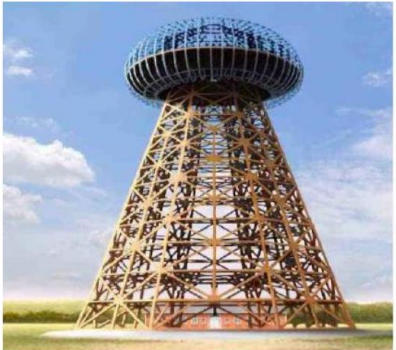
\includegraphics[width=0.5\textwidth]{tour_tesla} \end{center} \ \\
	Au fil du XXe siècle, bien que la recherche sur le WPT ait été mise en veilleuse pendant certaines périodes, surtout avec la montée des technologies de câbles électriques, l'intérêt a été ravivé dans les années 1960. William C. Brown, un pionnier du WPT, a mené des expérimentations avec des tubes micro-ondes, développant une antenne rectificatrice capable de convertir l'énergie électromagnétique en électricité. Ses travaux ont démontré que, même sur de longues distances, il était possible de transmettre efficacement de l'énergie.\\
	
	Dans les années 1980 et 1990, des recherches intensives ont été menées dans des domaines tels que l'induction magnétique et la résonance magnétique. Ces technologies ont permis de considérer le WPT non seulement pour des applications industrielles, mais aussi pour des dispositifs grand public tels que les chargeurs sans fil pour smartphones et accessoires.\\
	
	Aujourd'hui, le WPT est en pleine expansion, soutenu par le développement de l'Internet des Objets (IoT) et par la nécessité d'alimenter de manière efficace et durable une multitude d'appareils connectés. Grâce aux contributions de pionniers tels que Nikola Tesla, l'évolution des technologies de WPT continue de façonner notre façon d'interagir avec l'énergie, offrant un avenir où la recharge sans fil pourrait devenir la norme.
	
	
	\newpage
	\section{Classification des techniques de WPT}
	
	Pour mieux appréhender les différentes approches du transfert d’énergie sans fil (WPT), il est pertinent de les regrouper selon le principe physique sous-jacent utilisé pour assurer la transmission. Deux grandes catégories se dégagent généralement : les méthodes basées sur l’induction magnétique et celles basées sur le couplage capacitif. Chacune de ces techniques présente des avantages et des limites spécifiques, en fonction de la distance de transmission, de la puissance requise ou encore du contexte d’application. La suite de cette section détaille ces différentes méthodes.
	
	\subsection{Méthodes basées sur l’induction magnétique}
	Les méthodes basées sur l'induction magnétique utilisent des champs magnétiques pour transférer l'énergie.\\
	
	Le  modèle de $WPT$ basé sur l'induction magnétique se présente de la manière suivante:\\
	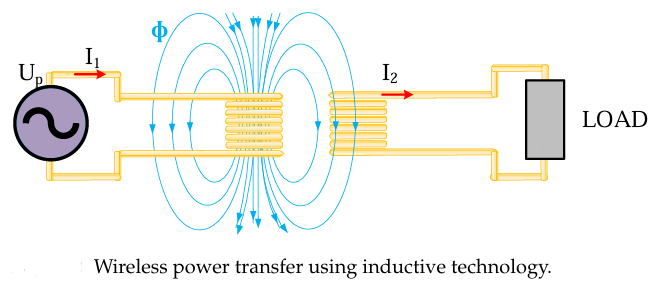
\includegraphics[width=0.9\textwidth]{WPT_inductif} \\ En voici le schémas bloc:\\
	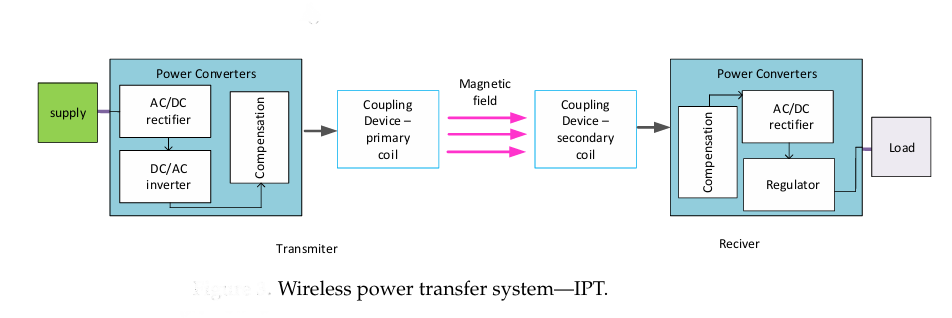
\includegraphics[width=1.1\textwidth]{WPT_inductif_1}
	
	Voici quelques modèles basés sur la transmission d'énergie sans fil par induction magnétique:
	\begin{itemize}
		\item Induction magnétique classique
		\item Résonance magnétique
		\item Ondes radio-fréquence
		\item Micro-ondes
		\item Laser ou infrarouge
	\end{itemize}
	\subsubsection{Induction magnétique classique}
	Cette méthode repose sur le principe fondamental de l’induction électromagnétique découvert par Faraday. Un courant alternatif circulant dans une bobine primaire (émettrice) génère un champ magnétique variable. Ce champ induit une tension dans une bobine secondaire (réceptrice), permettant ainsi le transfert d’énergie sans contact.
	
	Cette méthode est la plus couramment utilisée dans les chargeurs de smartphones, les brosses à dents électriques, etc. Elle est efficace à très courte distance (quelques centimètres) et nécessite un bon alignement des bobines.
	\paragraph{Principe: \\}
	Cette méthode utilise un champ magnétique variable généré par une bobine primaire alimentée en courant alternatif. Ce champ induit un courant dans une bobine secondaire proche, permettant un transfert d’énergie sans fil.
	\paragraph{Distance efficace: \\}
	Quelques millimètres à 5 $cm$
	\paragraph{Gamme de fréquence: \\}
	20 $KHz$ à 500 $KHz$
	\paragraph{Avantages: }
	\begin{itemize}
		\item Simplicité de conception
		\item Très efficace sur courte distance
		\item sécuritaire (faible champ rayonné)
	\end{itemize}
	\paragraph{Inconvénients: }
	\begin{itemize}
		\item Faible portée
		\item Sensible à l’alignement des bobines
		\item Faible tolérance au désalignement
	\end{itemize}
	
	
	\subsubsection{Résonance magnétique}
	La résonance magnétique est une amélioration de l’induction classique. Elle utilise deux circuits résonants (c’est-à-dire qui oscillent à la même fréquence naturelle) pour optimiser le couplage magnétique entre émetteur et récepteur, même à une distance plus grande (plusieurs dizaines de centimètres à mètres).
	
	Cette technologie est prometteuse pour la recharge de véhicules électriques ou de dispositifs médicaux.
	\paragraph{Principe: \\}
	Deux circuits (émetteur et récepteur) résonnent à la même fréquence naturelle, maximisant le transfert d’énergie même à distance plus grande que l’induction classique.
	\paragraph{Distance efficace: \\}
	10 $cm$ à 2 $m$
	\paragraph{Gamme de fréquence: \\}
	100 $kHz$ à 10 $MHz$
	\paragraph{Avantages: }
	\begin{itemize}
		\item Portée plus grande que l’induction classique
		\item Bonne efficacité même avec désalignement
		\item Adaptée à des systèmes mobiles (robots, véhicules)
	\end{itemize}
	\paragraph{Inconvénients: }
	\begin{itemize}
		\item Plus complexe à concevoir
		\item Coûteux (composants résonants de précision)
		\item Sensible à la variation de la fréquence de résonance
	\end{itemize}



	\subsubsection{Ondes radio-fréquences}
	Le transfert d’énergie par ondes RF utilise des antennes pour émettre des ondes électromagnétiques captées par un récepteur (rectenna). Bien que la puissance transférée soit faible, cette méthode est utilisée dans l’alimentation de capteurs IoT ou de tags RFID.
	\paragraph{Principe: \\}
	Le transfert d’énergie est réalisé via des ondes électromagnétiques radio émises par une antenne et reçues par une antenne (rectenna) qui convertit l’énergie en courant continu.
	\paragraph{Distance efficace: \\}
	1 $m$ à plusieurs mètres (jusqu’à 10 $m$ voire plus)
	\paragraph{Gamme de fréquence: \\}
	3 $kHz$ à 300 $GHz$ \\ (typique : 900 $MHz$ ou 2.4 $GHz$ pour IoT)
	\paragraph{Avantages: }
	\begin{itemize}
		\item Grande portée
		\item Non directionnel (pas besoin d’alignement précis)
		\item Intégration facile dans les objets connectés
	\end{itemize}
	\paragraph{Inconvénients: }
	\begin{itemize}
		\item Très faible rendement (1 à 5 \% souvent)
		\item Puissance transférable très faible (mW)
		\item Soumis à réglementation stricte des ondes RF
	\end{itemize}

	\subsubsection{Micro-ondes}
	Le principe est semblable aux RF mais avec une fréquence plus élevée, permettant une concentration d’énergie plus importante. Les micro-ondes sont utilisées pour le transfert longue distance, comme dans les projets spatiaux (alimentation de satellites).
	\paragraph{Principe: \\}
	Semblable aux RF, mais à fréquence plus élevée. Les ondes sont dirigées via des antennes vers un récepteur, souvent utilisé dans des applications longue distance à haute puissance.
	\paragraph{Distance efficace: \\}
	Plusieurs mètres à kilomètres (ligne de vue)
	\paragraph{Gamme de fréquence: \\}
	300 $MHz$ à 300 $GHz$ \\ (typiquement 2.45 $GHz$, 5.8 $GHz$)
	\paragraph{Avantages: }
	\begin{itemize}
		\item Transfert à longue distance
		\item Bonne directionnalité du faisceau
		\item Efficacité correcte avec bon alignement
	\end{itemize}
	\paragraph{Inconvénients: }
	\begin{itemize}
		\item Risques biologiques (échauffement)
		\item Coût élevé
		\item Nécessite un alignement précis
	\end{itemize} 

	\subsubsection{Laser ou infrarouge}
	Le transfert d’énergie par laser ou infrarouge repose sur un faisceau lumineux cohérent (laser) ou un rayonnement infrarouge dirigé vers un photo-détecteur. Il permet de transmettre de l’énergie sur de longues distances avec une haute précision.
	\paragraph{Principe: \\}
	Un faisceau lumineux (laser ou infrarouge) est émis vers un photodétecteur qui convertit l’énergie lumineuse en électricité. Utilisé pour les grandes distances avec besoin de précision.
	\paragraph{Distance efficace: \\}
	Jusqu’à plusieurs kilomètres (ligne de vue)
	\paragraph{Gamme de fréquence: }
	\begin{itemize}
		\item \textbf{Infrarouge:} 300 $GHz$ – 400 $THz$
		\item \textbf{Laser:} 30 $THz$ – 300 $THz$
	\end{itemize}
	\paragraph{Avantages: }
	\begin{itemize}
		\item Très grande portée
		\item Transfert directionnel très efficace
		\item Peu de pertes hors du faisceau
	\end{itemize}
	\paragraph{Inconvénients: }
	\begin{itemize}
		\item Risques pour les yeux (sécurité laser)
		\item Fonctionne uniquement en ligne de vue
		\item Coût élevé des dispositifs optiques
	\end{itemize}
	
	\subsection{Méthodes basées sur le couplage capacitif}
	Les méthodes basées sur le transfert capacitif utilisent des champs électriques ou des faisceaux lumineux.
	
	Le  modèle de $WPT$ basé sur l'induction magnétique se présente de la manière suivante:\\
	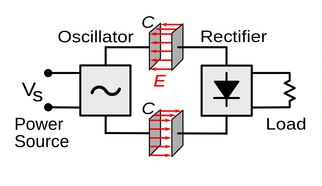
\includegraphics[width=0.53\textwidth]{WPT_capacitif} 
	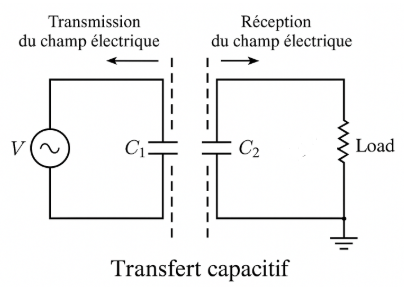
\includegraphics[width=0.47\textwidth]{WPT_capacitif_3}
	\\ En voici le schémas bloc:\\
	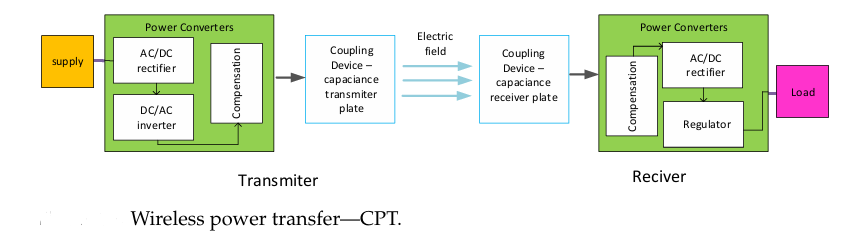
\includegraphics[width=1.1\textwidth]{WPT_capacitif_1}
	
	Cette méthode repose sur un champ électrique oscillant généré entre deux électrodes (plutôt que magnétique). Elle convient bien aux courtes distances et à des milieux où les champs magnétiques sont perturbés (médical, capteurs, etc.).
	
	Elle est très utilisée dans les implants médicaux, interfaces tactiles, ou certaines solutions IoT.
	\paragraph{Principe: \\}
	Le transfert d’énergie capacitif repose sur la création d’un champ électrique oscillant entre deux plaques conductrices (ou électrodes), séparées par un milieu isolant (diélectrique). Une tension alternative appliquée entre les électrodes génère un champ électrique variable qui transmet l’énergie vers la plaque réceptrice.
	\paragraph{Composants principaux: }
	\begin{itemize}
		\item Deux électrodes conductrices (plaques d’aluminium, cuivre ou PCB).
		\item Une source de tension alternative (générateur AC ou oscillateur).
		\item Un circuit de redressement (pont de diodes), un condensateur de filtrage et une charge.
	\end{itemize}
	\paragraph{Transmission et réception du champ électrique: }
	\begin{itemize}
		\item L’émetteur applique une tension AC sur la première plaque : champ électrique créé.
		\item Le champ traverse le diélectrique (air, tissu, etc.).
		\item La deuxième plaque (réceptrice) capte ce champ, provoquant un déplacement de charges qui est converti en courant utilisable.
	\end{itemize}
	\paragraph{Distance efficace: \\}
	1 $mm$ à 5 $cm$
	\paragraph{Gamme de fréquence: \\}
	500 $kHz$ à 40 $MHz$
	\paragraph{Avantages: }
	\begin{itemize}
		\item Pas de champ magnétique (pas de perturbation Électromagnétique)
		\item Composants miniatures (applications médicales)
		\item Moins sensible à l’orientation
	\end{itemize}
	\paragraph{Inconvénients: }
	\begin{itemize}
		\item Puissance transférée limitée
		\item Tensions élevées requises
		\item Forte sensibilité à l’environnement (humidité, diélectrique)
	\end{itemize}

	
	\subsection*{*Remarques}
	La transmission par couplage inductif et capacitif est une classification en tenant compte du mode de couplage, cela n'est pas le seul mode de  classification pouvant être utiliser, une des autres méthodes de classification est en foction de la distance. En tenant compte de la distance nous avons:
	\begin{itemize}
		\item \textbf{Champ lointain} (Par Laser et par micro-onde)
		\item \textbf{Champ proche} (Par induction, par résonance,et par capacité )
	\end{itemize}

	\section*{*Graphique illustratif}
	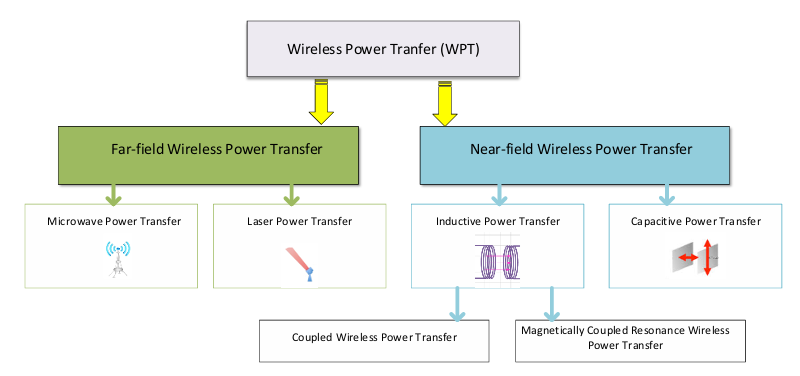
\includegraphics[width=1.1\textwidth]{classification_WPT}
	
	
	
	
	
	\section{Simulation sur Simulink}
	
	Dans le but de mieux illustrer le fonctionnement d’un système de transfert d’énergie sans fil (WPT), une simulation a été réalisée à l’aide du logiciel Simulink. Cette simulation permet non seulement de visualiser le comportement dynamique du système, mais également d’en évaluer les performances selon différents paramètres. Elle offre un aperçu concret de la manière dont les lois théoriques du WPT s’appliquent dans une configuration pratique. Dans les sections suivantes, nous décrivons les objectifs de la simulation, les choix techniques effectués, ainsi que les résultats obtenus et leur interprétation.
	
	\subsection{Objectif de la simulation}
	
	L’objectif est de modéliser un système de transfert d’énergie sans fil (WPT) basé sur le couplage inductif résonant dans Simulink. Cette simulation permettra :
	
	\begin{itemize}
		\item de visualiser le comportement dynamique du transfert d’énergie ;
		\item d’évaluer les performances de rendement ;
		\item d’analyser l’influence de la distance de couplage (inductance mutuelle) ;
		\item de suivre les tensions et courants dans les éléments émetteurs et récepteurs.
	\end{itemize}
	
	\subsection{Schéma du système WPT à simuler}
	
	Le modèle Simulink est basé sur les composants suivants :
	\begin{itemize}
		\item une source AC sinusoïdale (100 kHz) ;
		\item un circuit LC série (L1, C1) pour la bobine émettrice ;
		\item un couplage mutuel entre les bobines (Mutual Inductor) ;
		\item un circuit LC (L2, C2) résonant côté réception ;
		\item un pont de diodes pour le redressement ;
		\item un condensateur de filtrage ;
		\item une charge résistive (RL).
	\end{itemize}
	
	Voici le schéma utilisé pour la manipulation sur Simulink:\\
	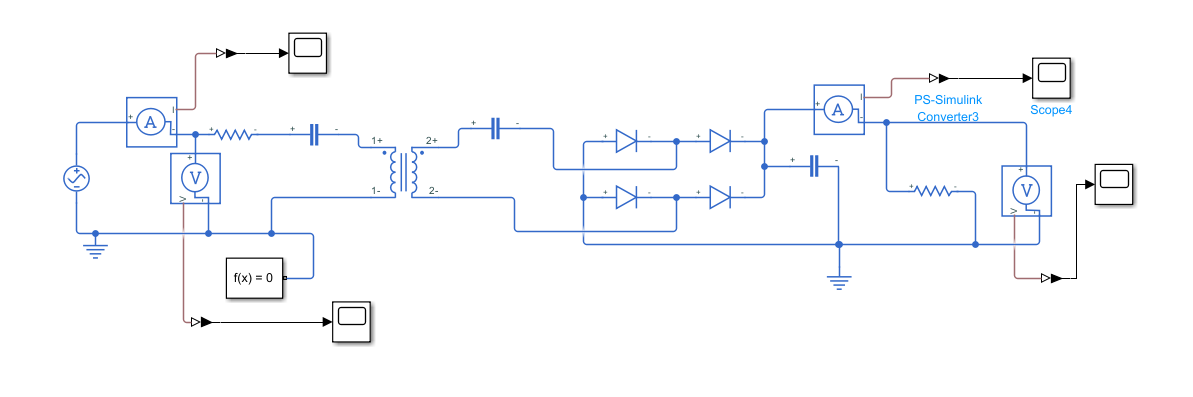
\includegraphics[width=1\textwidth]{WPT_simul}\\
	
	
	\subsection{Paramètres de simulation}
	Pour tester le schémas, voici les paramètres des composants ayant été utilisé.
	\begin{itemize}
		\item Tension de la source : $v = 12\ \text{Volts} $
		\item Fréquence de la source : $f = 100\ \text{kHz}$
		\item Inductances : $L_1 = L_2 = 100\ \mu H$
		\item Capacité de résonance : $C = \frac{1}{(2\pi f)^2 L} \approx 25.3\ \text{nF}$
		\item Résistance primaire : $R_L = 10\ \Omega$
		\item Résistance de la charge : $R_L = 10\ \Omega$
		\item Couplage : $k = 0.5$ (modifiable pour tester différentes distances)
	\end{itemize}
	
	\subsection{Justification du choix des composants et des valeurs}
	\begin{itemize}
		\item \textbf{Fréquence de la source ($100 kHz$):} Cette fréquence se situe dans la plage typique des systèmes WPT à courte distance, offrant un bon compromis entre compacité des composants et réduction des pertes.
		\item \textbf{Inductances L1 et L2 ($100\ \mu H$) :} Ces valeurs sont adaptées pour obtenir, avec un condensateur choisi correctement, une résonance à la fréquence de 100 kHz.
		\item  \textbf{Condensateur  $C \approx 25.3\ nF$:} découle de la formule de la résonance:  $$C = \frac{1}{(2\pi f)^2 L}$$
		\item \textbf{Couplage $K=\ 0.5$:} Représente un couplage moyen, permettant d'étudier l'effet de la distance sur le rendement. La valeur de k est modulable pour analyse.
		
		Soit $d$(la distance entre les deux bobines) et $r$(le rayon de la bobine, si on considère que les deux bobines sont identiques pour simplifier les calculs).
		
		Pour le cas $d >> r$ on a $k \approx \frac{\pi \ r4}{d^3 \sqrt{\mu_o \epsilon_o}}$, ceci veut dire que \textbf{la valeur de k est inversement proportionnelle à la distance entre les bobines.}
		\item \textbf{Charge RL ($10 \Omega$) :} Une valeur standard permettant une visualisation claire de la tension et du courant du côté récepteur.
	\end{itemize}
	
	
	\subsection{Étapes de la simulation}
	
	\begin{enumerate}
		\item Construction du circuit dans Simulink avec les blocs de \textit{Simscape Electrical}.
		\item Connexion de l’inductance mutuelle via le bloc \textit{Mutual Inductor}.
		\item Simulation en régime permanent avec différentes valeurs de $k$ (ou $M$).
		\item Visualisation des courbes de tension, courant et puissance via les blocs \textit{Scope}.
		\item L'ajout des certains blocs nécessaires pour une manipulation Simulink
	\end{enumerate}
	
	\subsection{Résultats attendus}
	
	\begin{itemize}
		\item Évolution des tensions et courants côté émission et réception.
		\item Analyse de la puissance transférée selon la variation de la distance.
		\item Courbes rendement = $\frac{P_{sortie}}{P_{entrée}} \times 100\%$
	\end{itemize}
	
	Une fois que le programme est lancé, voici les résultats que l'on obtient:
	
	\paragraph{La tension au primaire\\}
	Voici la courbe de la tension alternatif et sinusoïdale fournie par la source\\ 
	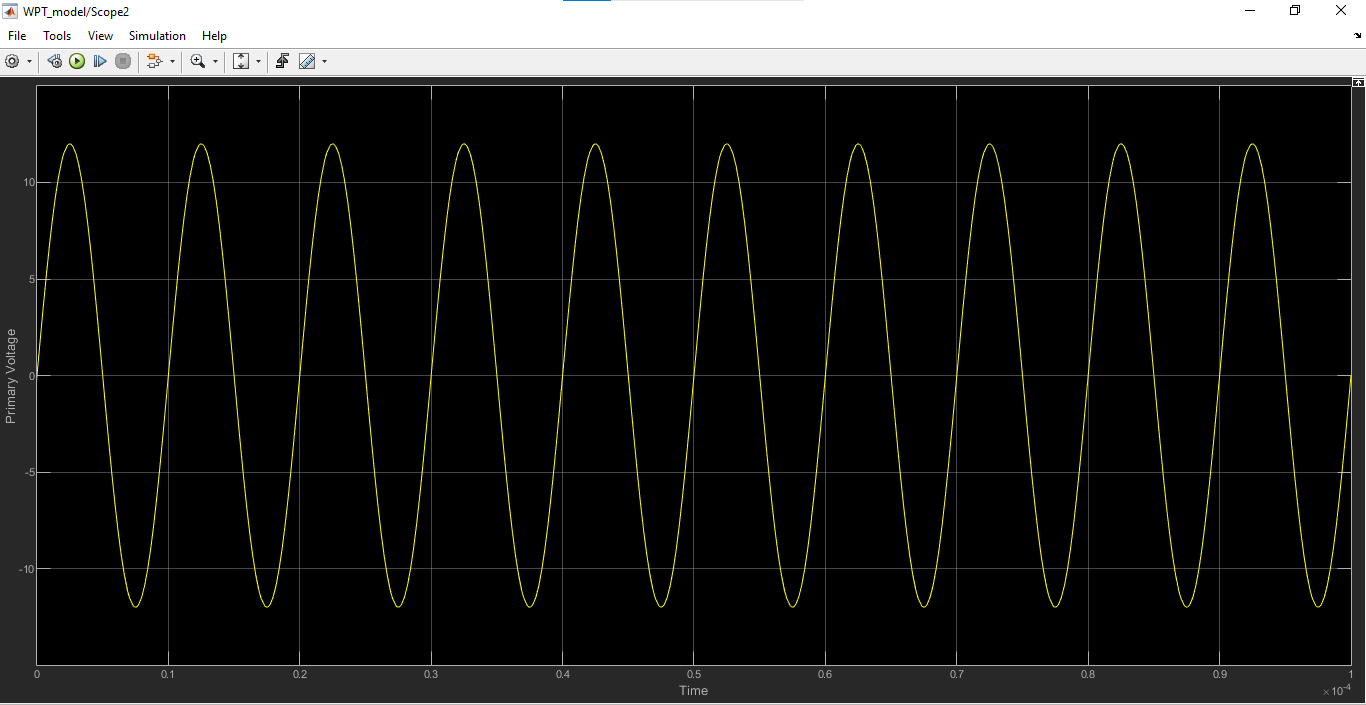
\includegraphics[width=1\textwidth]{WPT_simul_pv}
	
	\paragraph{Le courant au primaire\\}
	Voici la courbe du courant alternatif fournie par la source\\ 
	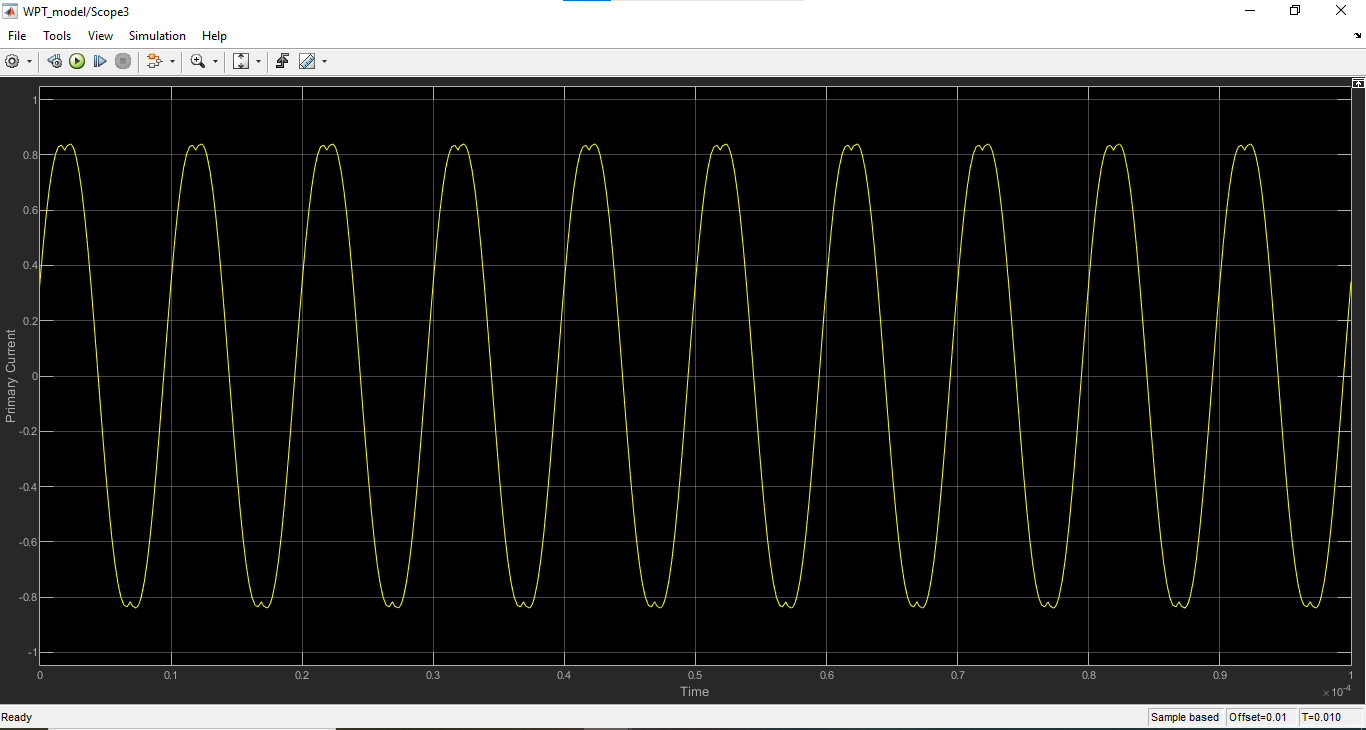
\includegraphics[width=1\textwidth]{WPT_simul_pc}
	\paragraph{La tension au secondaire\\}
	Voici la courbe de la tension après le redressement au coté secondaire, on voit bien que ce dernier n'a pas d'oscillation importante à cause de la présence du condensateur de filtrage et du pont des diodes\\ 
	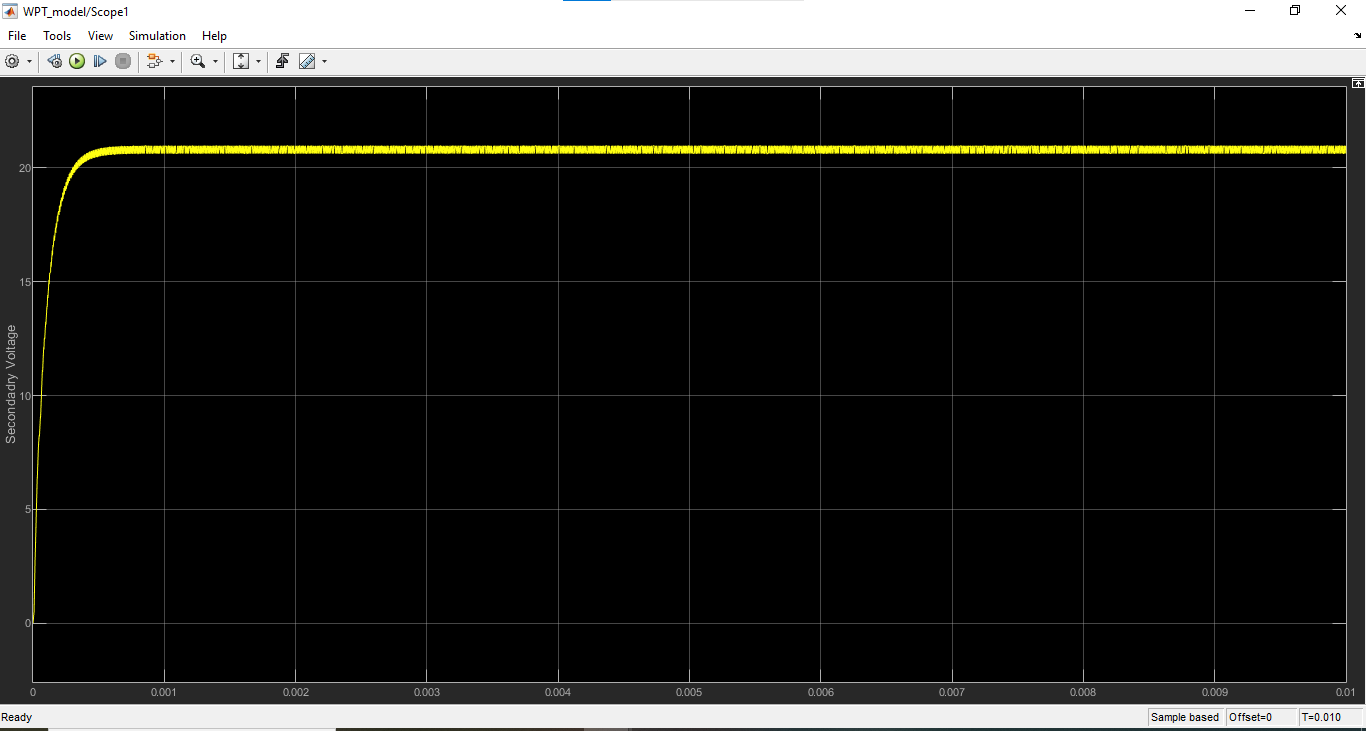
\includegraphics[width=1\textwidth]{WPT_simul_sv}
	
	\paragraph{Le courant au secondaire\\}
	Voici la courbe du courant au secondaire, ce dernier n'étant pas alternatif oscille quand même du coté positif\\ 
	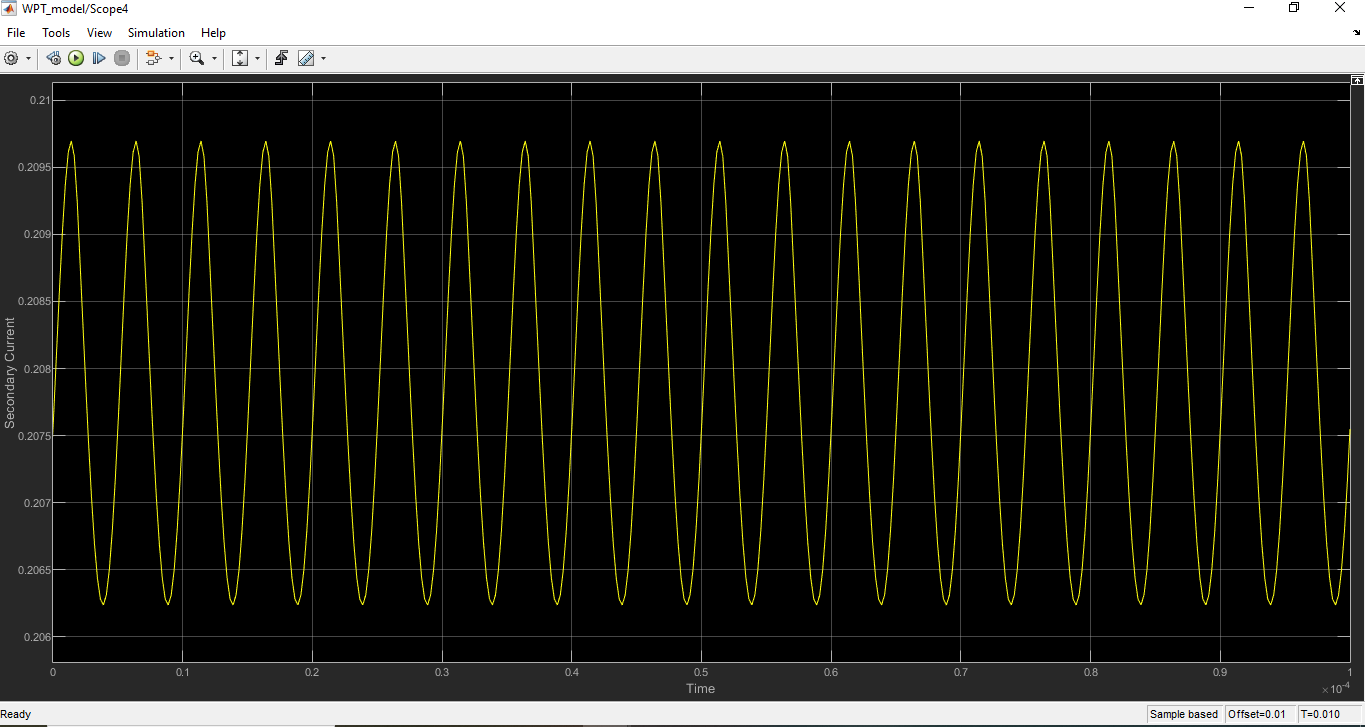
\includegraphics[width=1\textwidth]{WPT_simul_sc}
	
	\subsubsection*{Influence de la distance}
	Pour pouvoir l'influence de la distance sur le rendement d'un système WPT inductif, on va varier le coefficient de couplage $k$ et prélevé la puissance d'entrée et de sortie à chaque fois tout en vérifiant la variation du rendement par rapport au coefficient de couplage.\\
	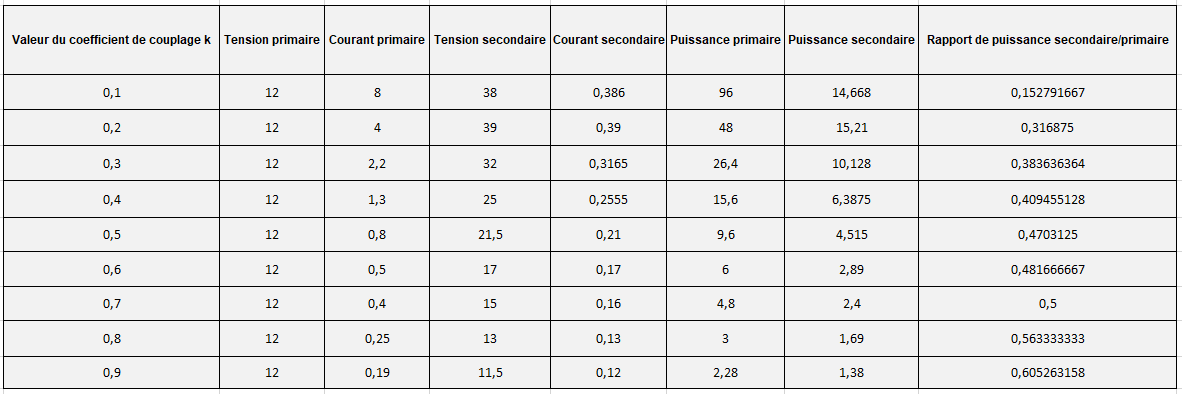
\includegraphics[width=1\textwidth]{WPT_simul_gain}\\
	
	\
	\\
	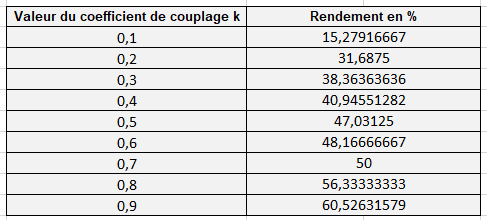
\includegraphics[width=1\textwidth]{WPT_simul_gain1}\\
	On remarque que plus on augmente le coefficient de couplage, plus le rendement aussi augmente; autrement nous pouvont dire que lorsque la distance entre les bobines diminue, le rendement augmente. 
	
	\subsubsection*{Courbe du rendement}
	Voici une courbe du rendement par rapport au coefficient de couplage(la distance)\\
	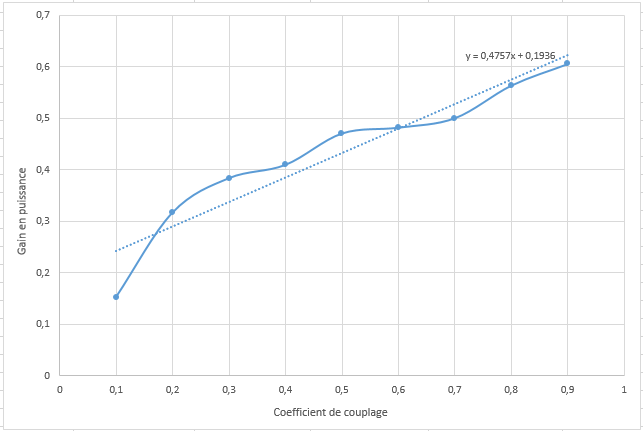
\includegraphics[width=1\textwidth]{WPT_simul_gain_graph}\\
	
	
	\subsection{Discutions}
	
	Le rendement observé dans notre simulation varie entre 15 \% et 60 \% selon le coefficient de couplage.
	
	D’après [Coca, 2016] et les publications IEEE (ex. : \textbf{Detka} \& \textbf{Górecki}, 2022), les systèmes WPT inductifs résonants atteignent des rendements typiques de 70 \% à 95 \% à courte distance.
	Notre simulation reste donc dans une plage acceptable, bien que certains cas réels optimisés dépassent les 90 \%.\\
	
	Des chercheurs ont publié une étude sur \textit{l'étude de la transmission d'energie sans fil $WPT$ basée sur la résonance couplée magnétique.}
	
	Voici l'image du montage qu'ils ont réalisé:\\
	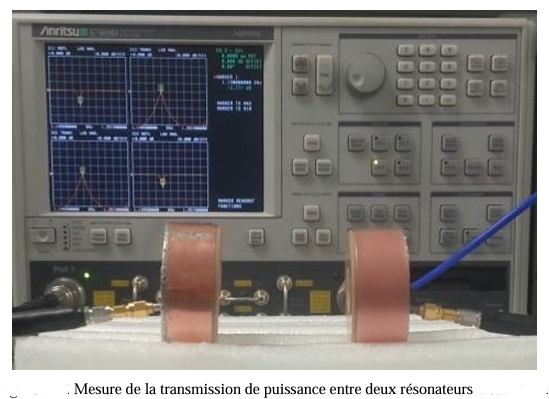
\includegraphics[width=1\textwidth]{WPT_disc}\\
	
	
	Voici une image du rendement en fonction de la distance qu'ils ont obtenu:\\
	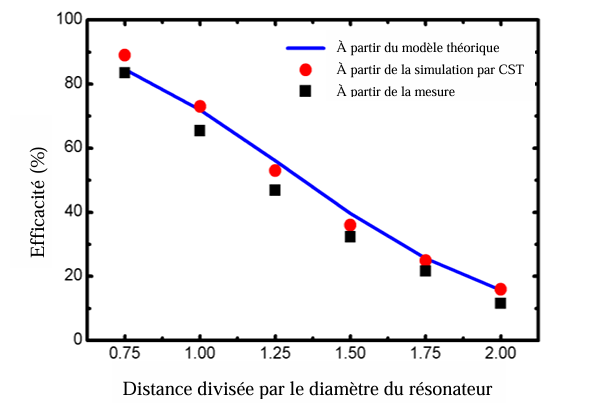
\includegraphics[width=1\textwidth]{WPT_disc_1}\\
	D'après cette étude, le rendement varie en fonction de la distance , et ce rendement va de 20 à 80\%, pour une fréquence de $1,2 \ GHZ$.  
	
	
	
	
	
	\section{Lois physiques utilisées et leurs applications dans le WPT}
	Le Wireless Power Transfer repose sur des lois fondamentales de l’électromagnétisme. Ces lois permettent de modéliser le comportement des champs magnétiques et électriques nécessaires à la transmission d’énergie sans fil.
	
	\subsection{Loi de Faraday}
	\textbf{Énoncé :} Toute variation du flux magnétique à travers une boucle de conducteur génère une force électromotrice (fem) dans cette boucle.
	
	\textbf{Formule :}
	\[
	E = -\frac{d\Phi_B}{dt}
	\]
	où :
	\begin{itemize}
		\item \(E\) est la fem (en volts)
		\item \(\Phi_B\) est le flux magnétique (en Weber, Wb)
	\end{itemize}
	
	\textbf{Application dans le WPT :} Dans les systèmes à induction magnétique, un courant alternatif dans la bobine émettrice crée un champ magnétique variable. Ce champ traverse la bobine réceptrice, et selon la loi de Faraday, y induit un courant électrique. C’est le principe fondamental du transfert d’énergie inductif.
	
	\subsection{Loi d’Ampère-Maxwell}
	\textbf{Énoncé :} Le champ magnétique est généré par un courant électrique ou par une variation du champ électrique.
	
	\textbf{Formule (forme intégrale) :}
	\[
	\oint \vec{B} \cdot d\vec{l} = \mu_0 I + \mu_0 \epsilon_0 \frac{d\Phi_E}{dt}
	\]
	où :
	\begin{itemize}
		\item \(\vec{B}\) est le champ magnétique
		\item \(I\) est le courant traversant la surface
		\item \(\frac{d\Phi_E}{dt}\) est le taux de variation du flux électrique
		\item \(\mu_0\) et \(\epsilon_0\) sont les constantes du vide
	\end{itemize}
	
	\textbf{Application dans le WPT :} Dans les systèmes à couplage capacitif, une variation de champ électrique crée aussi un champ magnétique selon cette loi. Cela permet un couplage alternatif à celui basé sur les bobines, en utilisant plutôt des électrodes planes.
	
	\subsection{Principe de résonance}
	\textbf{Énoncé :} Lorsque deux circuits ont la même fréquence de résonance, le transfert d’énergie entre eux est maximal.
	
	\textbf{Formule de la fréquence de résonance d’un circuit LC :}
	\[
	f_0 = \frac{1}{2\pi\sqrt{LC}}
	\]
	où :
	\begin{itemize}
		\item \(L\) est l’inductance (en Henry)
		\item \(C\) est la capacité (en Farad)
	\end{itemize}
	
	\textbf{Application dans le WPT :} Utilisé dans la résonance magnétique, ce principe permet de maximiser le transfert d’énergie sur des distances moyennes. Deux circuits RLC, accordés à la même fréquence, peuvent échanger de l’énergie de manière efficace même s’ils ne sont pas parfaitement alignés.
	
	\section{Coefficient de couplage}
	\textbf{Définition :} Le coefficient de couplage, noté \(k\), est un paramètre qui mesure le degré de couplage entre deux éléments inductifs (bobines) ou capacitifs (électrodes). Il indique combien de flux magnétique ou de champ électrique produit par l’émetteur est capté par le récepteur.
	
	\textbf{Formule :}
	\[
	k = \frac{M}{\sqrt{L_1 L_2}}
	\]
	où :
	\begin{itemize}
		\item \(M\) est l’inductance mutuelle entre les deux bobines (en Henry)
		\item \(L_1\) et \(L_2\) sont les inductances propres des deux bobines
	\end{itemize}
	
	\textbf{Valeur de \(k\) :}
	\begin{itemize}
		\item \(k = 1\) : couplage parfait (tout le flux est capté)
		\item \(k \approx 0\) : pas de couplage (aucun transfert)
	\end{itemize}
	
	\textbf{Fonctionnement et impact :} Un \(k\) élevé signifie que la bobine réceptrice capte efficacement le champ généré, ce qui améliore le rendement du système. Un \(k\) faible indique un désalignement, une trop grande distance, ou des pertes importantes.
	
	Le coefficient de couplage dépend de :
	\begin{itemize}
		\item La distance entre les éléments
		\item L’alignement
		\item La géométrie des bobines ou électrodes
		\item Le milieu environnant (air, diélectrique)
	\end{itemize}
	
	\textbf{Utilisation dans le WPT :} Dans l’induction magnétique, \(k > 0.7\) est généralement requis pour un transfert efficace. En résonance magnétique, \(k\) peut être faible (0.1–0.5) mais la résonance permet de compenser. En couplage capacitif, le coefficient dépend de la capacité mutuelle entre les plaques.
	
	
	
	
	
	
	
	
	
	\section{Applications des systèmes de transfert d'énergie sans fil (WPT)}
	
	Les systèmes de transfert d'énergie sans fil ($WPT$) ont un large éventail d'applications dans divers domaines. Cette section explore certaines de ces applications, mettant en avant leurs potentiels et leurs impacts.
	
	\subsection{Chargement sans fil d'appareils électroniques}
	
	L'une des applications les plus populaires du WPT est le chargement sans fil des appareils électroniques tels que les smartphones, tablettes et montres connectées. Grâce à la technologie Qi, par exemple, les utilisateurs peuvent recharger leurs appareils en les plaçant simplement sur un pad de chargement, éliminant ainsi le besoin de câbles et ports de connexion.
	
	\subsection{Véhicules électriques}
	
	Le WPT est en train de transformer le secteur des transports, notamment avec l'émergence de solutions de chargement sans fil pour les véhicules électriques. Cela inclut :
	\begin{itemize}
		\item \textbf{Chargement statique} : Les véhicules stationnés peuvent se recharger sans avoir à brancher un câble.
		\item \textbf{Chargement dynamique} : Des infrastructures routières intégrant des bobines $WPT$ permettent de recharger les véhicules en mouvement, augmentant ainsi leur autonomie sans frais d'exploitation.
	\end{itemize}
	
	\subsection{Applications industrielles}
	
	Dans le secteur industriel, le WPT offre des solutions pour recharger des capteurs, des équipements robotiques et d'autres appareils sans fil. Cela permet de réduire les coûts d'entretien liés aux fils et connecteurs, tout en augmentant la sécurité dans des environnements potentiellement dangereux.
	
	\subsection{Applications médicales}
	
	Les systèmes WPT trouvent également leur place dans le domaine médical, permettant le rechargement sans fil d'appareils implantables tels que les stimulateurs cardiaques et les dispositifs de surveillance. Cette technologie permet d'améliorer le confort des patients tout en réduisant la nécessité de procédures chirurgicales pour remplacer les batteries.
	
	\subsection{Domotique et Internet des objets (IoT)}
	
	Avec l'explosion des dispositifs IoT, le WPT constitue une solution efficace pour alimenter de nombreux appareils domestiques, tels que les capteurs de sécurité, les thermostats intelligents et autres gadgets connectés. L'utilisation du WPT facilite l'intégration et le déploiement de ces appareils sans fil dans notre vie quotidienne.
	
	\subsection{Conclusion sur les applications}
	
	Les applications des systèmes de WPT sont vastes et en constante évolution. Avec les progrès technologiques et l'augmentation de la demande pour des solutions d'alimentation sans fil, l'avenir du WPT semble prometteur, offrant des gains d'efficacité et de commodité dans de nombreux domaines.
	
	\section{Avantages et inconvénients des systèmes WPT}
	
	Les systèmes de transfert d'énergie sans fil ont des avantages significatifs ainsi que certaines limitations. Cette section examine en détail ces aspects.
	
	\subsection{Avantages}
	
	\begin{itemize}
		\item \textbf{Commodité} : L'élimination des câbles de chargement et de connexion rend l'utilisation plus pratique, surtout pour les appareils portables.
		\item \textbf{Sécurité} : Réduit les risques de chocs électriques et d'accidents liés aux câbles, en particulier dans des environnements humides ou industriels.
		\item \textbf{Flexibilité d'installation} : Permet une intégration facile dans divers environnements sans les contraintes des connexions câblées.
		\item \textbf{Maintenance réduite} : Moins de pièces mobiles et d'interfaces physiques réduisent le besoin de maintenance et de réparations fréquentes.
	\end{itemize}
	
	\subsection{Inconvénients}
	
	\begin{itemize}
		\item \textbf{Efficacité énergétique} : Les systèmes WPT peuvent avoir des pertes d'énergie significatives, surtout sur de longues distances.
		\item \textbf{Coûts d'installation} : Le coût initial d'installation de ces systèmes peut être élevé, limitant leur adoption dans certaines applications.
		\item \textbf{Portée limitée} : L'efficacité de la transmission d'énergie diminue avec l'augmentation de la distance entre la source et le récepteur.
		\item \textbf{Interférences électromagnétiques} : Les systèmes WPT peuvent interférer avec d'autres dispositifs électroniques, ce qui peut poser des problèmes de compatibilité.
	\end{itemize}
	
	\subsection{Conclusion sur les avantages et inconvénients}
	
	En conclusion, bien que les systèmes de transfert d'énergie sans fil offrent de nombreux avantages en termes de commodité et de sécurité, ils présentent également des défis qui doivent être pris en compte, notamment l'efficacité énergétique et le coût. Une évaluation soigneuse est nécessaire pour déterminer leur adéquation pour des applications spécifiques.
	
	\section{Recherches actuelles, innovations et perspectives d'avenir}
	
	Voici un aperçu des recherches récentes dans le domaine des systèmes de transfert d'énergie sans fil, ainsi que des innovations marquantes et des perspectives d'avenir pour cette technologie.
	
	\subsection{Recherches actuelles}
	
	Les travaux récents se concentrent sur plusieurs axes d'amélioration, notamment :
	\begin{itemize}
		\item \textbf{Efficacité énergétique} : Des recherches sont en cours pour améliorer l'efficacité des systèmes WPT par l'optimisation des conceptions de bobines et des algorithmes de contrôle.
		\item \textbf{Intégration avec les technologies IoT} : La convergence des systèmes WPT avec les technologies de l'Internet des objets est un domaine actif, visant à alimenter des dispositifs connectés sans fil dans des environnements domestiques et industriels.
		\item \textbf{Développement de nouveaux matériaux} : L'utilisation de matériaux avancés pour les bobines et les systèmes d'absorption d'énergie est également explorée pour optimiser la performance.
	\end{itemize}
	
	\subsection{Innovations}
	
	Certaines innovations récentes dans le domaine se distinguent :
	\begin{itemize}
		\item \textbf{Chargement dynamique des véhicules} : Des projets pilotes pour le chargement de véhicules électriques en mouvement émergent, avec des technologies adaptées intégrées dans les infrastructures routières.
		\item \textbf{Systèmes de recharge pour appareils médicaux} : L'intégration du WPT dans les dispositifs médicaux implantables permet une recharge sans intervention chirurgicale, améliorant ainsi la qualité de vie des patients.
		\item \textbf{Technologies de résonance magnétique} : Avancées dans les systèmes à résonance magnétique permettant des distances de transfert d'énergie plus longues tout en maintenant une haute efficacité.
	\end{itemize}
	
	\subsection{Perspectives d'avenir}
	
	À l'avenir, le WPT pourrait :
	\begin{itemize}
		\item \textbf{Devenir omniprésent} : Avec l'amélioration continue des technologies, le WPT pourrait être intégré dans une variété d'applications, rendant les dispositifs omniprésents encore plus pratiques.
		\item \textbf{Évoluer vers des solutions non intrusives} : La recherche vise à rendre les systèmes de WPT plus discrets, permettant une intégration dans des environnements quotidiens sans compromettre l'esthétique.
		\item \textbf{Répondre aux exigences énergétiques croissantes} : À mesure que le nombre d'appareils connectés augmente, le WPT pourrait jouer un rôle crucial dans la gestion et la distribution d'énergie, surtout dans les villes intelligentes.
	\end{itemize}
	
	\newpage
	\section{Conclusion}
	
	
	
	
	

	
	\newpage
	\section*{Bibliographie}
	\addcontentsline{toc}{section}{Bibliographie}
	\vspace{1cm}
	\begin{itemize}
		\item EM - Notes de base.pdf : notes du cours d'électromagnétisme 2021
		\item Coca, E. (Éd.). (2016). Wireless Power Transfer: Fundamentals and Technologies.
		\item IJETT. (2016). Revue de l'IJETT sur la WPT.
		\item IEEE Spectrum. (2023). It’s Time to Rethink 6G.
		\item Detka, K., \& Górecki, K. (2022). Wireless Power Transfer—A Review. Energies, 15(7236).
		\item Etude Electromagnétique du Transfert Sans Fil d’Energie par voie de Couplage Inductif Résonant Série-Parallèle .pdf : mémoire
		\item Huang, L., \& Hu, A.P. (2015). Defining the mutual coupling of capacitive power transfer for wireless power transfer. Electronics Letters.
		\item https://theorycircuit.com/wireless/wireless-power-transmitter-and-receiver-circuit/
		\item https://publications.polymtl.ca/1496/1/2014\_WeiWang.pdf
		\item http://large.stanford.edu/courses/2016/ph240/arshavsky1/
		\item Kenneth R.Demarest, “Engineering Electromagnetics”, Prentice Hall, 1997. 
		\item  Chi Wang Zaki, K.A., “Dielectric resonators and filters,” Microwave Magazine, IEEE, 
		Vol.8, Issue: 5, pp.115-227, Oct. 2007
		\item  A. S. Y. Poon, "Electromagnetic field focusing for short-range wireless power 
		transmission," in 2012 6th IEEE Radio and Wireless Week, RWW 2012 - 2012 IEEE 
		Radio and Wireless Symposium, RWS 2012, January 15, 2012 - January 18, 2012, Santa 
		Clara, CA, United states, 2012, pp. 115-118. 
		\item S. Kim, J. S. Ho, L. Y. Chen, and A. S. Y. Poon, "Wireless power transfer to a cardiac 
		implant," Applied Physics Letters, vol. 101, 2012. 
		\item Qi standard ”System Description Wireless Power Transfer Vol. I: Low Power” [online], 
		available: http://www.wirelesspowerconsortium.com 
		
			
	\end{itemize}
	
	
	
	
	
	
	
	
	
	
	
	
	
	
	
	
	
	
	
	
	
	
	
	
	
	
	
	
	
	
\end{document}	